
\chapter{Diseño e implementación} % Main chapter title
En este capítulo se abordará la descripción de la arquitectura general del sistema, arquitectura del firmware, código de los controladores desarrollados, desarrollo del hardware y la configuración de la plataforma IoT.
\label{Chapter3} % Change X to a consecutive number; for referencing this chapter elsewhere, use \ref{ChapterX}

\definecolor{mygreen}{rgb}{0,0.6,0}
\definecolor{mygray}{rgb}{0.5,0.5,0.5}
\definecolor{mymauve}{rgb}{0.58,0,0.82}

%%%%%%%%%%%%%%%%%%%%%%%%%%%%%%%%%%%%%%%%%%%%%%%%%%%%%%%%%%%%%%%%%%%%%%%%%%%%%
% parámetros para configurar el formato del código en los entornos lstlisting
%%%%%%%%%%%%%%%%%%%%%%%%%%%%%%%%%%%%%%%%%%%%%%%%%%%%%%%%%%%%%%%%%%%%%%%%%%%%%
\lstset{ %
  backgroundcolor=\color{white},   % choose the background color; you must add \usepackage{color} or \usepackage{xcolor}
  basicstyle=\footnotesize,        % the size of the fonts that are used for the code
  breakatwhitespace=false,         % sets if automatic breaks should only happen at whitespace
  breaklines=true,                 % sets automatic line breaking
  captionpos=b,                    % sets the caption-position to bottom
  commentstyle=\color{mygreen},    % comment style
  deletekeywords={...},            % if you want to delete keywords from the given language
  %escapeinside={\%*}{*)},          % if you want to add LaTeX within your code
  %extendedchars=true,              % lets you use non-ASCII characters; for 8-bits encodings only, does not work with UTF-8
  %frame=single,	                % adds a frame around the code
  keepspaces=true,                 % keeps spaces in text, useful for keeping indentation of code (possibly needs columns=flexible)
  keywordstyle=\color{blue},       % keyword style
  language=[ANSI]C,                % the language of the code
  %otherkeywords={*,...},           % if you want to add more keywords to the set
  numbers=left,                    % where to put the line-numbers; possible values are (none, left, right)
  numbersep=5pt,                   % how far the line-numbers are from the code
  numberstyle=\tiny\color{mygray}, % the style that is used for the line-numbers
  rulecolor=\color{black},         % if not set, the frame-color may be changed on line-breaks within not-black text (e.g. comments (green here))
  showspaces=false,                % show spaces everywhere adding particular underscores; it overrides 'showstringspaces'
  showstringspaces=false,          % underline spaces within strings only
  showtabs=false,                  % show tabs within strings adding particular underscores
  stepnumber=1,                    % the step between two line-numbers. If it's 1, each line will be numbered
  stringstyle=\color{mymauve},     % string literal style
  tabsize=2,	                   % sets default tabsize to 2 spaces
  title=\lstname,                  % show the filename of files included with \lstinputlisting; also try caption instead of title
  morecomment=[s]{/*}{*/}
}


%----------------------------------------------------------------------------------------
%	SECTION 1
%----------------------------------------------------------------------------------------
\section{Diagrama de bloques general del sistema}

En la figura \ref{fig:Diagrama general del sistema IoT} se muestra el diagrama en bloques general del sistema donde se describe la arquitectura IoT aplicada al trabajo que consta de tres capas: percepción, red y aplicación.

\begin{figure}[h]
	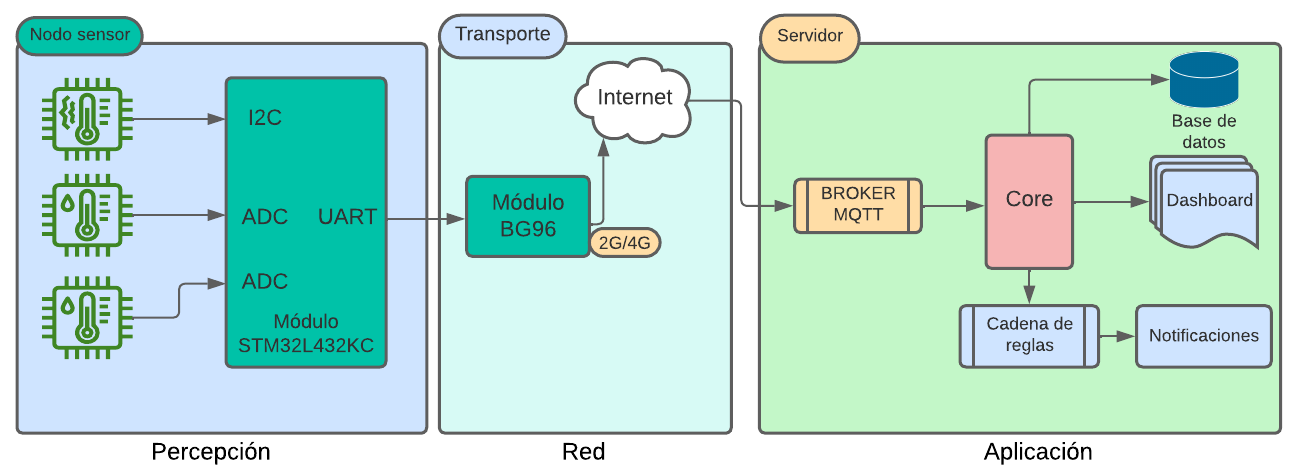
\includegraphics[width=\textwidth, height=8cm]{./Figures/DiagramaDelSistema.png}
	\caption{Diagrama general del sistema IoT.}
	\label{fig:Diagrama general del sistema IoT}
\end{figure}

En cada una de las capas se despliegan tecnologías y componentes de hardware y software. A continuación se describe cada una de las capas.

\begin{itemize}
	\item Capa de percepción: en la capa de percepción se encuentra el nodo sensor que es el encargado de medir las variables físicas, hacer un preprocesamiento y posteriormente enviar los datos a la capa de red. Para su desarrollo se utilizó la tarjeta de prueba STM32L432KC que contiene el firmware del sistema, además, se utilizaron los siguientes sensores: sensor de humedad y temperatura ambiente AHT10, sensor de humedad de suelo HL-69 y el sensor de luz UV ML8511.
  \item Capa de red: en lo que respecta a la conectividad de red, se empleó un módulo Quectel BG96 que es capaz de establecer conexión de manera automática con las redes 2G, 4G y NB-IoT, según las condiciones de red en el lugar de implementación del nodo sensor. Este módulo se comunica con el microcontrolador mediante comandos AT a través del puerto UART.
  \item Capa de aplicación: en la capa de aplicación, se utilizó ThingsBoard como plataforma IoT que brinda los microservicios de broker MQTT como puerta de entrada al servidor, base de datos para el almacenamiento, interfaz gráfica para la visualización de los datos y permite gestionar las alarmas del sistema.
\end{itemize}

\section{Arquitectura de firmware}
El desarrollo del firmware fue la tarea más compleja del trabajo debido a que uno de los objetivos fue lograr un firmware estructurado en capas para facilitar el desarrollo y reducir la complejidad del código. La figura \ref{fig:Capas del firmware} muestra la división en capas del firmware desarrollado.

\begin{figure}[h]
  \centering
	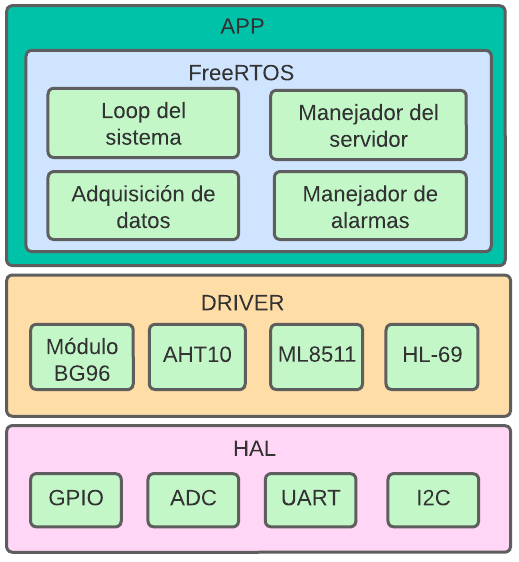
\includegraphics[width=7cm, height=8cm]{./Figures/Capas del firmware.png}
	\caption{Capas del firmware.}
	\label{fig:Capas del firmware}
\end{figure}

\subsection{Capa HAL} 
La capa HAL (\textit{Hardware Abstraction Layer}) proporcionada por el fabricante del microcontrolador  es la más baja del sistema, proporciona a las capas superiores la capacidad de interactuar con los periféricos del  microcontrolador a través de funciones en lenguaje C.
\begin{itemize}
  \item GPIO: la API proporciona funciones  para gestionar las entradas y salidas del microcontrolador. Fueron utilizadas por la capa de APP para el control de los leds de debug y para el encendido y reset del módulo de comunicación.
  \item ADC: proporcionan funciones para la configuración, lectura y escritura de los pines del microcontrolador para trabajar con señales analógicas. Se utilizaron estas funciones para hacer la lectura de los sensores de humedad del suelo y el sensor de luz UV.
  \item UART: brinda funciones para la lectura y escritura del puerto UART del microcontrolador. El firmware utiliza estas funciones para la comunicación con el módulo BG96.
  \item I2C: proporciona funciones para la lectura y escritura por protocolo I2C. El driver del sensor AHT10 utiliza estas funciones para hacer la lectura de los datos.
\end{itemize}

\subsection{Capa drivers} 
La capa drivers (manejador de dispositivos) está compuesta por los manejadores que se desarrollaron para interactuar con el hardware externo al microcontrolador. Se desarrollaron dos drivers que se describen a continuación:
\begin{itemize}
  \item Driver BG96: las funciones más importantes que proporciona el driver son:
  \begin{itemize}
    \item Estado del módulo.
    \item Descripción del módulo.
    \item Configuración APN de la red.
    \item Conexión TCP.
    \item Conexión al broker MQTT.
  \end{itemize}
  \item Driver AHT10: se desarrollo utilizando la hoja de datos del sensor, proporciona funciones de inicialización y lectura de humedad y temperatura obtenidos por el sensor.
\end{itemize}
Para los sensores ML8511 y HL-69 que son sensores analógicos no se desarrollaron drivers, sino que se crearon funciones para convertir el valor analógico entregado a un valor significativo para el usuario con respecto a la variable física medida.
\subsection{Capa aplicación} 
La capa de APP o aplicación  es la de mayor nivel jerárquico. Se desarrolló sobre freeRTOS 
que permite hacer un código más escalable.

Se implementaron cuatro tareas.
\begin{itemize}
    \item Loop del sistema: esta tarea es la que brinda la secuencialidad del sistema.
    \item Manejador del  servidor: se encarga de manejar la conexión a la red y al broker MQTT.
    \item Adquisición de datos: se encarga de hacer la lectura de los sensores.
    \item Manejador de alarmas: esta tarea se encarga de hacer el control de las alarmas del sistema.
\end{itemize}
\clearpage

\section{Desarrollo del firmware}

Para el desarrollo del firmware se utilizó STM32CubeIDE que es el entorno de desarrollo oficial de STMicroelectronic.

El firmware fue desarrollado sobre freeRTOS, se utilizaron algunas de sus funcionalidades como colas, semáforos, tareas e interrupciones.

En la figura \ref{fig:Df inicio firmware}  se muestra en diagrama de flujo de inicialización del firmware.

\begin{figure}[htbp]
  \centering
	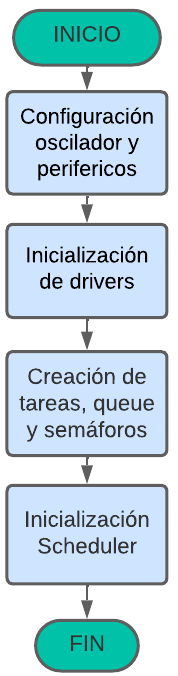
\includegraphics[width=2.5cm, height=9.5cm]{./Figures/DF inicio firmware.png}
	\caption{Diagrama de flujo de inicialización del firmware.}
	\label{fig:Df inicio firmware}
\end{figure}

Al iniciar el  firmware realiza la configuración del hardware del microcontrolador, inicializa los drivers del hardware externo, luego se crean los recursos del sistema operativo como tareas,colas y semáforos, finalmente se da el control del sistema al scheduler de freeRTOS. 

Para el control del sistema se crearon cuatro tareas sobre freeRTOS, que se comunican y sincronizan a través de colas y semáforos.

\subsection{Tarea loop del sistema} 

La secuencialidad del sistema es manejada por la tarea loop, la figura \ref{fig:Df tarea loop sistema} muestra el diagrama de flujo de la tarea loop.
La tarea comienza iniciando el timer del sistema el cual es el encargado de manejar el tiempo en que se repetira el ciclo de la tarea loop, luego la tarea se bloquea en el un semáforo que sera desbloqueada en el momento de la ejecución del handler de la interrupción del timer, luego se envia datos por la cola de adquisición de datos y server mqtt para levantar el servidor y la tarea se vuelve a bloquear en el semáforo, cuando se desbloquea pregunta si se logró levantar el servidor, si se logró se manda un mensaje por la cola de server mqtt con el evento de enviar datos y se bloquea nuevamente pero si no se logró levantar el servidor no se enviaran datos, luego se envía un evento a la cola de alarmas y  se bloquea nuevamente esperando que envíen las alarmas, cuando se desbloquea se manda un evento a la cola de server mqtt para desconectar el servidor y se bloquea la tarea en el semáforo esperando la desconexión  finalmente se inicia nuevamente el timer y mandamos al sistema a modo de bajo consumo.

\begin{figure}[h]  
\centering
	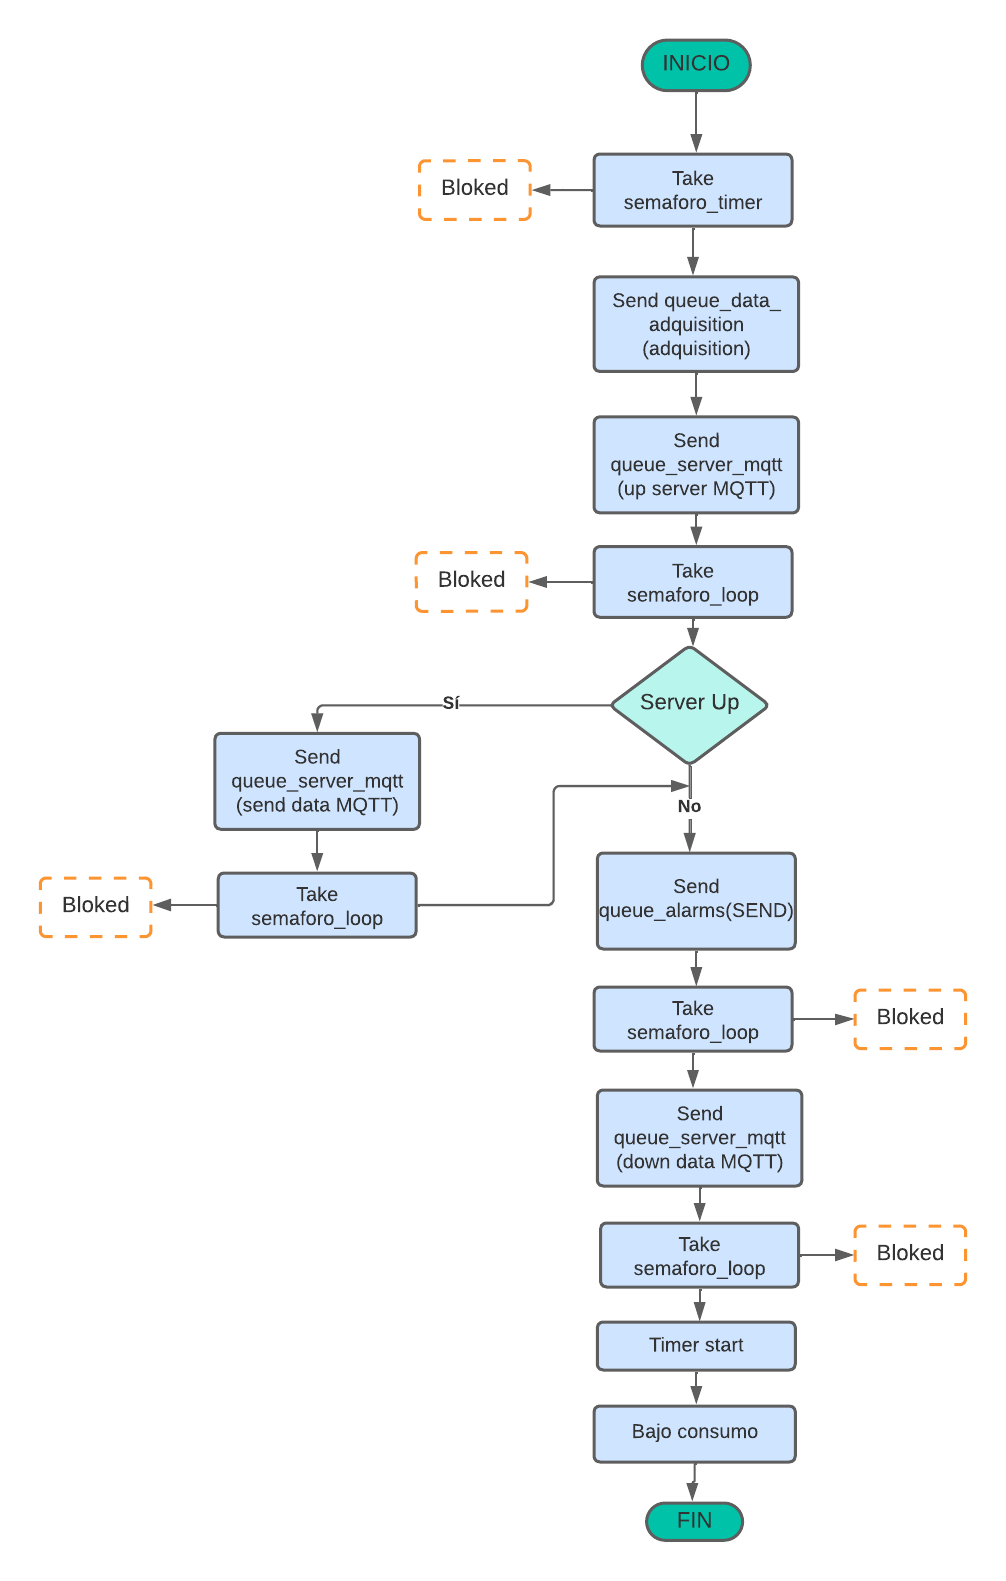
\includegraphics[width=12cm, height=16cm]{./Figures/DF task loop.png}
	\caption{Diagrama de flujo de la tarea loop.}
	\label{fig:Df tarea loop sistema}
\end{figure}

\subsection{Tarea adquisición de datos} 
La figura \ref{fig:Df tarea adquisicion} muestra el diagrama de flujo de la tarea de adquisición de datos. La tarea inicia revisando si hay datos en la cola de adquisición. Si existen datos, se realiza la lectura de todos los sensores para posteriormente enviar los  valores leídos por la cola de datos y alarmas. Si no hay datos en la cola la tarea se bloquea. 

\begin{figure}[h]
  \centering
	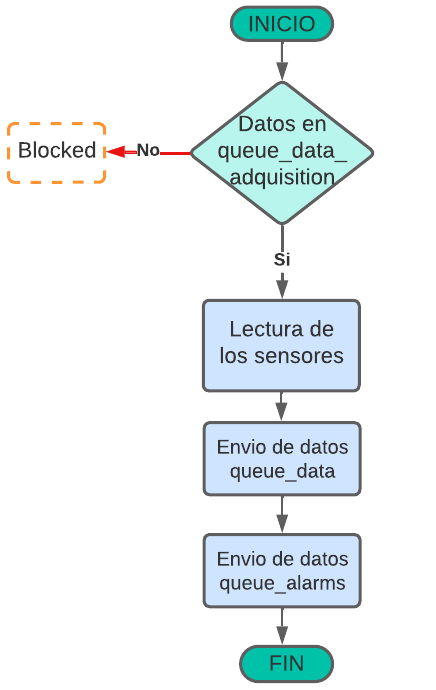
\includegraphics[width=5cm, height=7cm]{./Figures/DF task adquisicion.png}
	\caption{Diagrama de flujo tarea de adquisición de datos.}
	\label{fig:Df tarea adquisicion}
\end{figure}

\subsection{Tarea manejador de alarmas} 
El control de las alarmas se realiza a través una tarea del sistema operativo la figura \ref{fig:Df tarea alarmas} muestra el diagrama de flujo de la tarea de alarmas.

Al entrar al bucle infinito lo primero que realiza la tarea es revisar la cola de alarmas. Si existen datos se analiza el evento que contiene el dato recibido. Se tiene dos posibles eventos monitorear y enviar. Si el evento es monitorear se compara el valor del sensor de humedad con un valor mínimo permitido, si es menor se activa una alarma advierte al sistema que ocurrió esto a través de una variable. Si el evento es enviar se revisa si hay alarmas activas, enviando un mensaje de texto si así fuera. Si no hay datos en la cola de alarmas la tarea se bloquea. 

\begin{figure}[h]
  \centering
	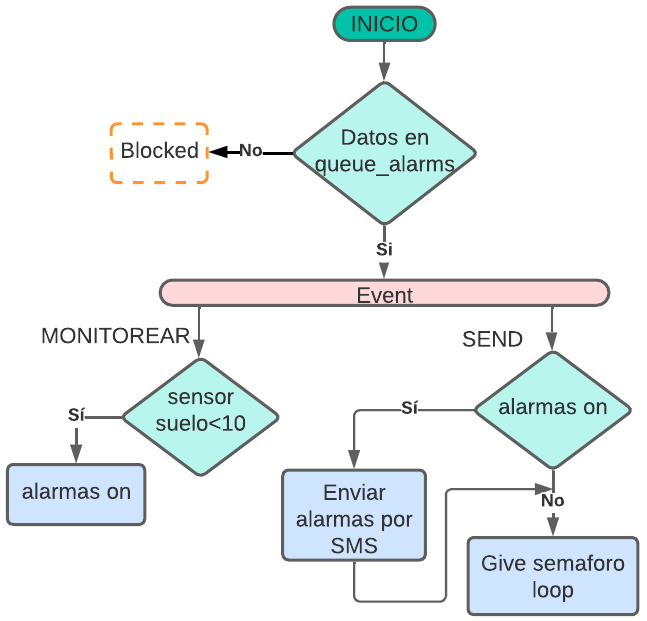
\includegraphics[width=6cm, height=6cm]{./Figures/DF_alarms.png}
	\caption{Diagrama de flujo de la tarea manejador de alarmas.}
	\label{fig:Df tarea alarmas}
\end{figure}

\subsection{Tarea manejador del servidor } 
La última tarea que se implementó es la tarea que maneja la conexión del servidor la figura \ref{fig:Df tarea conexion} muestra su diagrama flujo.

La tarea comienza esperando datos en la cola del servidor, al llegar datos se analiza el evento que se recibe. Se tiene tres posibles eventos UP, DOWN y SEND. Si el evento es UP la tarea entra a la máquina de estados que se muestra en la figura \ref{fig:Maquina de estados up servidor} que se utiliza para levantar una conexión con el servidor. Si el evento es DOWN la tarea ejecuta la máquina de estados que se ve en la figura \ref{fig:Maquina de estados dowm servidor} que se encarga de terminar la conexión con el servidor. Si el evento es SEND la tarea obtiene los últimos datos leídos por los sensores, armar la trama y publica los datos al broker MQTT. 
\begin{figure}[h]
  \centering
	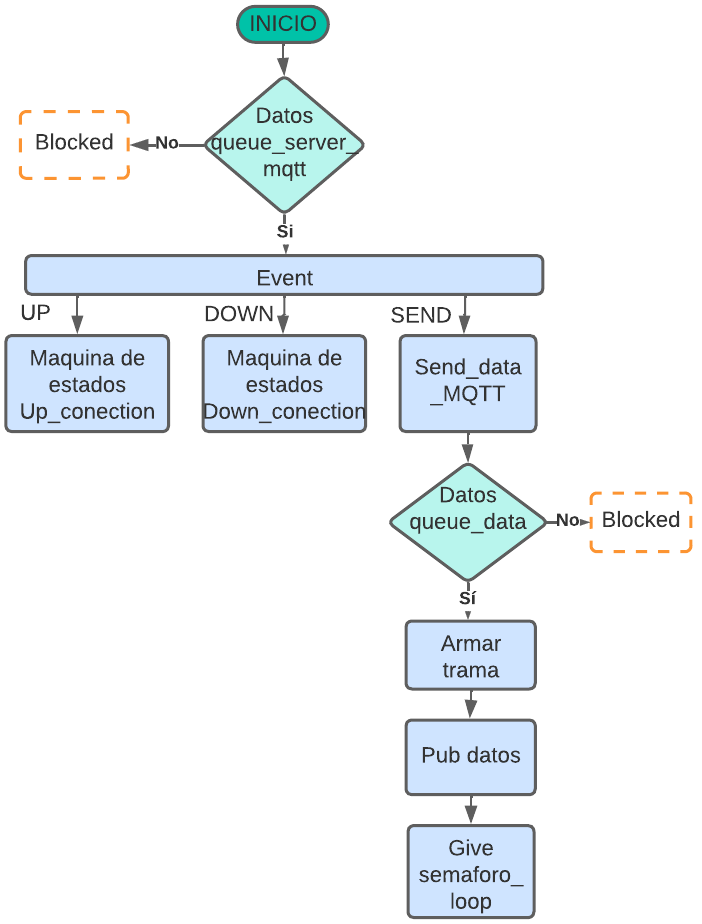
\includegraphics[width=8cm, height=8.5cm]{./Figures/DF general task conection.png}
	\caption{Diagrama de flujo de la tarea conexion server MQTT.}
	\label{fig:Df tarea conexion}
\end{figure}

\begin{figure}[h]
  \centering
  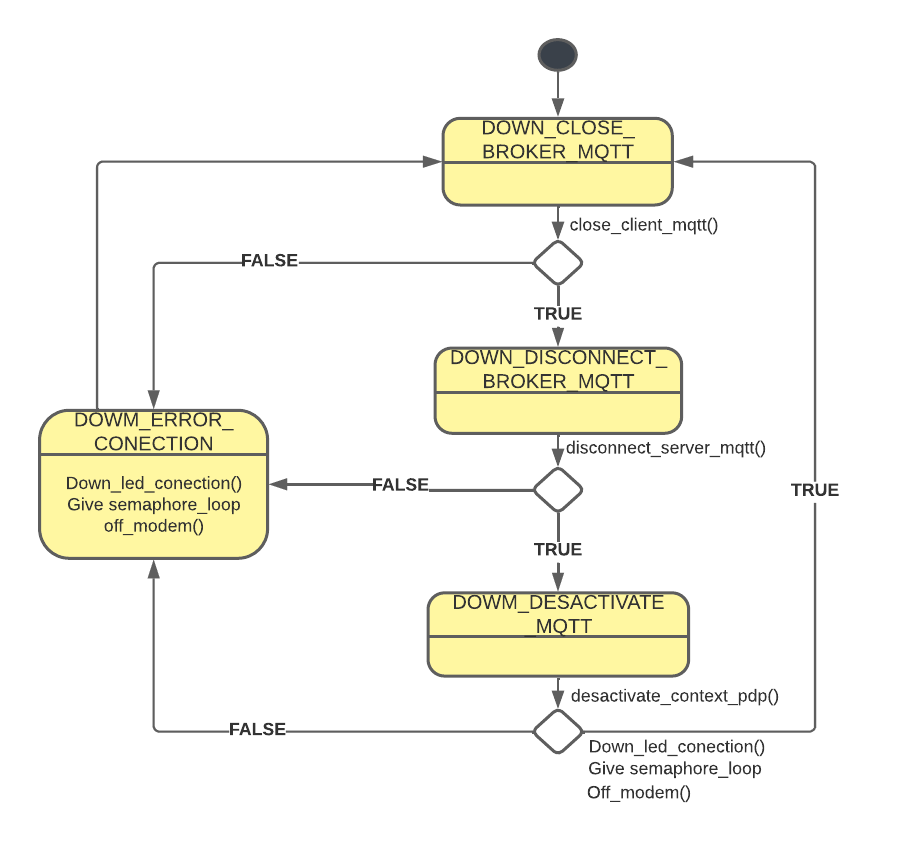
\includegraphics[width=8cm, height=8cm]{./Figures/SM down server.png}
  \caption{Máquina de estados down servidor.}
  \label{fig:Maquina de estados dowm servidor}
\end{figure}
\clearpage
\hspace{0.5cm}

\begin{figure}[t!]
  \centering
	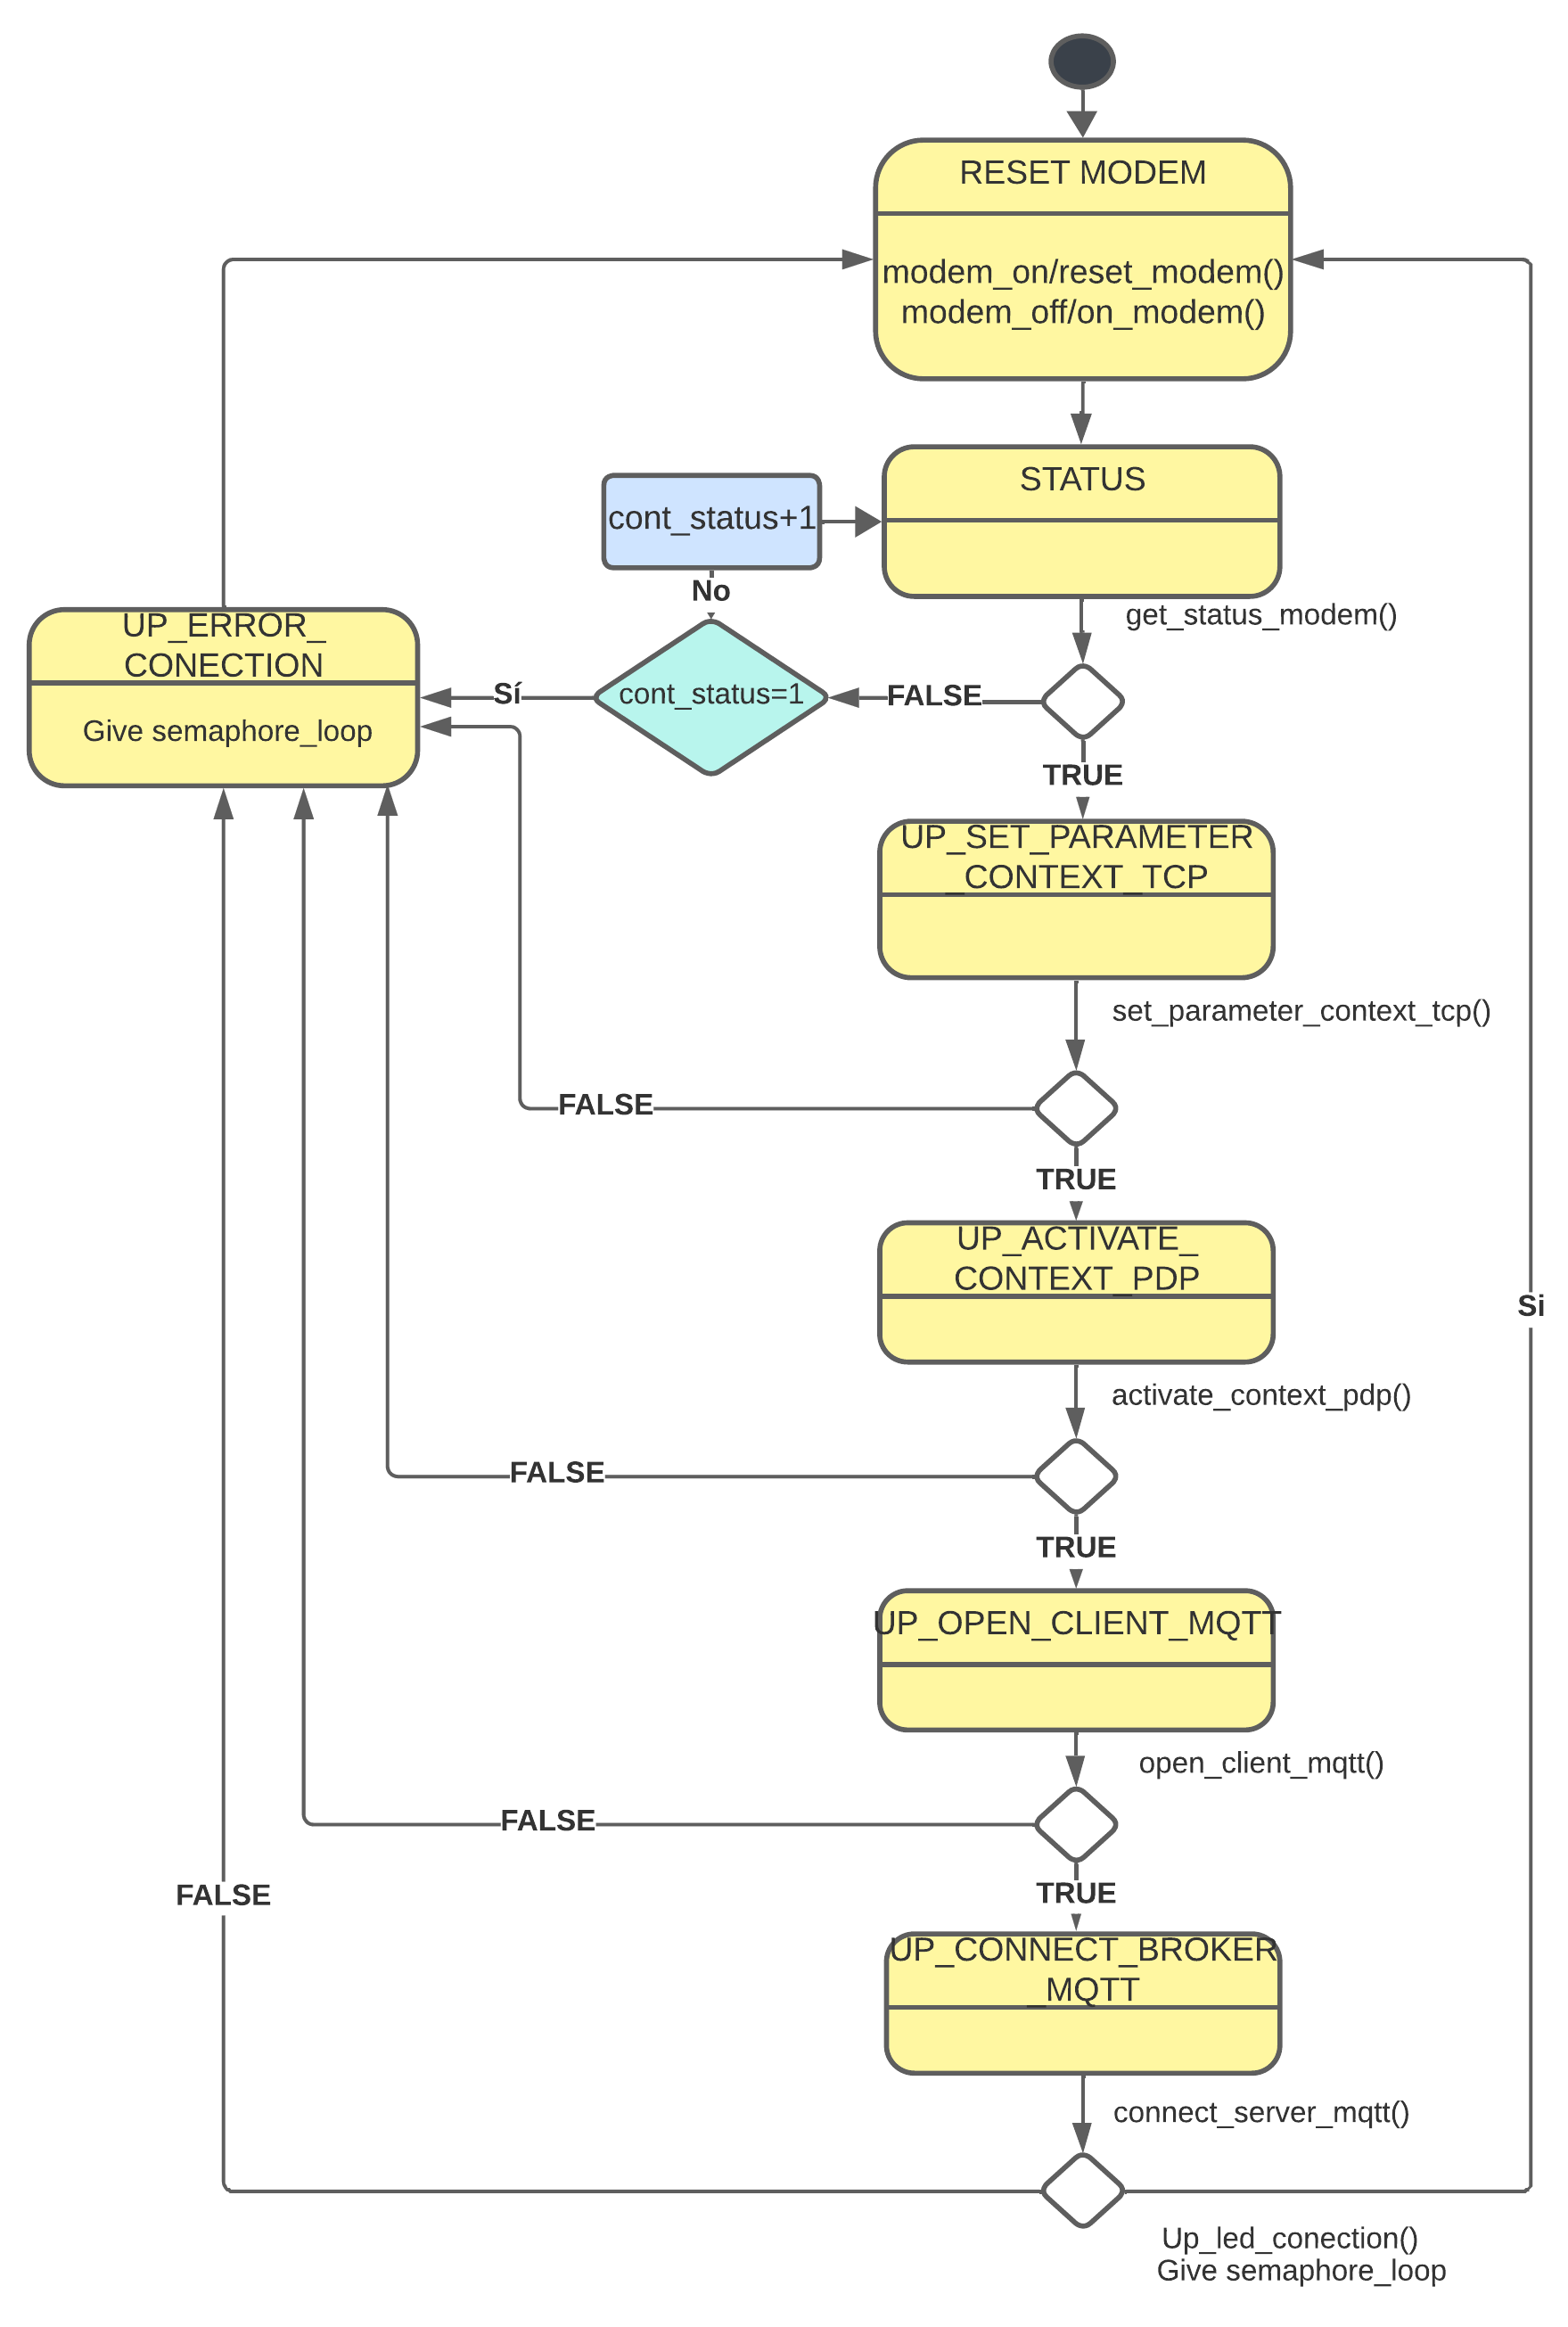
\includegraphics[width=10cm, height=14cm]{./Figures/SM up server.png}
	\caption{Máquina de estados up servidor.}
	\label{fig:Maquina de estados up servidor}
\end{figure}

\section{Controladores implementados}
Se implementaron dos controladores para el modulo de comunicacion BG96 y para el sensor de humedad y temperatura ambiente AHT-10.

\subsection{Controlador sensor AHT10} 
En el codigo \ref{cod:codigo AHT10} se ven las funciones mas utilizadas del driver en el firmware.

\begin{lstlisting}[label=cod:codigo AHT10,caption=Funciones principales del driver del sensor AHT10.]  % Start your code-block

//Estructura para manejar los datos del driver del sensor    
typedef struct 
{
  aht10WriteFcn_t  writeI2C;
  aht10ReadFcn_t  readI2C;
  delay1ms_t      delay_ms_I2C;    
  aht10_status_fnc status_fun;
}aht10_config_t;

//Funcion para inicializar el driver 
void aht10Init(aht10_config_t *obj, aht10WriteFcn_t fncWritePort, aht10ReadFcn_t fncReadPort, delay1ms_t fncDelayPort)
{
  obj->writeI2C=fncWritePort;
  obj->readI2C=fncReadPort;
  obj->delay_ms_I2C=fncDelayPort;
}
//Funcion para obtener el valor de la humedad
aht10_status_fnc aht10_get_humedity(aht10_config_t*obj, uint8_t *data)
{
  if (obj== NULL)
  {
    return AHT10_ERROR;
  }
  obj->status_fun=AHT10_ERROR;
  uint8_t bufferRead[6]={0};
  uint32_t data_humedity=0;
  obj->status_fun=aht10_launch_measurement(obj);
  if (obj->status_fun==AHT10_OK)
  {
    obj->status_fun= obj->readI2C(AHT10_ADDRESS_SLAVE,bufferRead,6);
    if (obj->status_fun==AHT10_OK)
    {
      data_humedity=(((uint32_t)bufferRead[1]<<16) | ((uint16_t)bufferRead[2]<<8) | (bufferRead[3]))>>4;
      *data= HUMEDITY(data_humedity);
    }
  }
  return obj->status_fun;
}
//Funcion para obtener el valor de la temperatura 
aht10_status_fnc aht10_get_temperature(aht10_config_t*obj, int8_t *data)
{
  if (obj== NULL)
  {
    return AHT10_ERROR;
  } 
  uint8_t buffer_read[6]={0};
  uint32_t data_temperature=0;
  obj->status_fun=AHT10_ERROR;
  obj->status_fun=aht10_launch_measurement(obj);
  if (obj->status_fun==AHT10_OK)
  {
    obj->status_fun=obj->readI2C(AHT10_ADDRESS_SLAVE ,buffer_read,6);
    if (obj->status_fun==AHT10_OK)
    {
      data_temperature=((uint32_t)(buffer_read[3] & 0x0F)<<16) | ((uint16_t) buffer_read[4]<<8)| buffer_read[5];
      *data= TEMPERATURE(data_temperature);
    }
  }
  return obj->status_fun;
}
\end{lstlisting}


\subsection{ Controlador módulo de comunicación BG96 } 
En el codigo \ref{cod:driver bg96} se muestran las funciones mas utilizadas por el firmware del driver que son las de configuracion y activacion del APN, conexion y desconexion al servidor MQTT.

\begin{lstlisting}[label=cod:driver bg96,caption=Funciones principales del driver del sensor AHT10.]  % Start your code-block

//Estructura para manejar los datos del driver 
typedef struct 
{
  em_status_modem  status_modem;
  em_state_server_mqtt_conection status_mqtt_server;
  pf_send_data    send_data_device;
  pf_reset_modem  f_reset_modem; 
  st_config_parameters_mqtt self_mqtt;
  st_config_context_tcp self_tcp;
  st_info_product info_product;
  uint8_t           last_error;
  char buffer_resp [100];
  char *current_cmd;
  em_bg96_error_handling ft_resp;
}st_bg96_config;

//Funcion de inicio del driver 
em_bg96_error_handling init_driver(st_bg96_config *self,pf_send_data ft_send_data_device,pf_reset_modem ft_reset_modem)
{
  if (ft_send_data_device!=NULL) {
    self->send_data_device=ft_send_data_device;
  }
  if (ft_reset_modem!=NULL) {
    self->f_reset_modem=ft_reset_modem;
  }
    self->status_modem=OFF;
    self->ft_resp=FT_BG96_OK;
    self->last_error=BG96_NO_ERROR;
    self->self_tcp.context_id=1;
    self->self_tcp.context_type=1;
    self->self_tcp.method_authentication=1;
    self->self_tcp.tcp_password="";
    self->self_tcp.tcp_username="";
    self->self_mqtt.identifier_socket_mqtt=0;
    self->self_mqtt.quality_service=0;
    self->self_mqtt.port=1883;
    self->self_mqtt.mqtt_client_id="123a56cb9";
    self->status_mqtt_server=SERVER_MQTT_DOWN;
    self->self_mqtt.host_name="\"mqtt.thingsboard.cloud\"";
    self->self_mqtt.mqtt_username="";
    self->self_mqtt.mqtt_password="";
    self->self_tcp.tcp_apn="internet.tigo.bol";
    return self->ft_resp;
}
//Funcion para obtener el estado del modulo
em_bg96_error_handling get_status_modem(st_bg96_config* self)
{
  self->ft_resp=FT_BG96_OK;
  self->current_cmd="AT\r";
  self->ft_resp=self->send_data_device(self->current_cmd,RS_BG96_OK,self->buffer_resp,1000);
  if (self->ft_resp!=FT_BG96_OK)
  {
    self->last_error=BG96_ERROR_STATUS_MODEM;
  }
  return self->ft_resp;
}
//Funcion para enviar mensaje de texto 
em_bg96_error_handling send_sms_bg96(st_bg96_config *self,char*number,char*message)
{
  self->ft_resp=FT_BG96_OK;
  char buffer_message[256];
  char buffer_number[20];
  sprintf(buffer_number,"AT+CMGS=\"%s\"\r",number);
  sprintf(buffer_message,"%s\x1a\r",message);
  
  self->ft_resp=self->send_data_device(buffer_number,RS_BG96_SIGNAL,self->buffer_resp,12000);
  if (FT_BG96_OK==self->ft_resp)
  {
    self->ft_resp=self->send_data_device(buffer_message,RS_BG96_OK,self->buffer_resp,12000);
    if (FT_BG96_OK!=self->ft_resp)
    {
      self->last_error=BG96_ERROR_SEND_SMS;
    }
  }
  return self->ft_resp;
}
//Funcion para configurar el contexto de la red
em_bg96_error_handling set_parameter_context_tcp(st_bg96_config *self)
{   
  self->ft_resp=FT_BG96_OK;
  char cmd[100];
  sprintf(cmd,"AT+QICSGP=%u,%u,\"%s\",\"%s\",\"%s\",%u\r",self->self_tcp.context_id,self->self_tcp.context_type,self->self_tcp.tcp_apn,self->self_tcp.tcp_username,self->self_tcp.tcp_password,self->self_tcp.method_authentication);
  self->ft_resp=self->send_data_device(cmd,RS_BG96_OK,self->buffer_resp,3000);
  if (self->ft_resp!=FT_BG96_OK)
  {
    self->last_error=BG96_ERROR_SET_PARAMETER_CONTEXT_TCP;
  }
  return self->ft_resp;
}
//Funcion para activar el contexto pdp
em_bg96_error_handling activate_context_pdp(st_bg96_config *self)
{
  self->ft_resp=FT_BG96_OK;
  char cmd[30];
  sprintf(cmd,"AT+QIACT=%u\r",self->self_tcp.context_id);
  self->ft_resp=self->send_data_device(cmd,RS_BG96_OK,self->buffer_resp,15000);
  if (self->ft_resp!=FT_BG96_OK)
  {
    self->last_error=BG96_ERROR_ACTIVATE_CONTEXT_PDP;
  }
  return self->ft_resp;
}
//Funcion para abrir un cliente MQTT
em_bg96_error_handling open_client_mqtt(st_bg96_config *self)
{
  self->ft_resp=FT_BG96_ERROR;
  char cmd[100];
  sprintf(cmd,"AT+QMTOPEN=%u,%s,%u\r",self->self_mqtt.identifier_socket_mqtt,self->self_mqtt.host_name,self->self_mqtt.port);
  self->ft_resp=self->send_data_device(cmd,RS_BG96_CERO,self->buffer_resp,75000);
  if (self->ft_resp!=FT_BG96_OK)
  {
    self->last_error=BG96_ERROR_OPEN_CLIENT_MQTT;
  } 
  return self->ft_resp;
}
//Funcion para conectarse al servidor MQTT
em_bg96_error_handling connect_server_mqtt(st_bg96_config *self)
{
  self->ft_resp=FT_BG96_ERROR;
  char cmd[150]={0};
  sprintf(cmd,"AT+QMTCONN=%u,\"%s\",\"%s\",\"%s\"\r",self->self_mqtt.identifier_socket_mqtt,self->self_mqtt.mqtt_client_id,self->self_mqtt.mqtt_username,self->self_mqtt.mqtt_password);
  self->ft_resp=self->send_data_device(cmd,RS_BG96_CERO,self->buffer_resp,10000);
  if (self->ft_resp!=FT_BG96_OK)
  {
    self->last_error=BG96_ERROR_CONNECT_SERVER_MQTT;
  }
  return self->ft_resp;
}
//Funcion para publicar un mensaje al topico configurado 
em_bg96_error_handling publish_message(st_bg96_config *self,char *topic,char *data)
{
  self->ft_resp=FT_BG96_ERROR;
  char cmd[50]={0};
  char buffer_data[220]={0};
  sprintf(buffer_data,"%s\x1a\r",data);
  sprintf(cmd,"AT+QMTPUB=%u,0,0,0,\"%s\"\r",self->self_mqtt.identifier_socket_mqtt,topic);
  self->ft_resp=self->send_data_device(cmd,RS_BG96_SIGNAL,self->buffer_resp,3000);
  if (FT_BG96_OK==self->ft_resp)
  {
    self->ft_resp=self->send_data_device(buffer_data,RS_BG96_CERO,self->buffer_resp,15000);
    if (self->ft_resp!=FT_BG96_OK)
    {
      self->last_error=BG96_ERROR_PUBLISH_MESSAGE;
    }   
 }
    else self->last_error=BG96_ERROR_PUBLISH_MESSAGE;
    return self->ft_resp;
}


\end{lstlisting}
\clearpage
\section{Desarrollo del hardware}

Para el diseño del hardware se empleó KiCad 6.0, una herramienta de diseño que se utilizó durante el desarrollo de la especialización.

\subsection{Esquemático} 
Al ser un prototipo lo que se hizo fue desarrollar un tarjeta donde se puedan ensamblar y conectar los módulos utilizados en el trabajo: módulo de comunicación celular, tarjeta de desarrollo con el microcontrolador y  los módulos sensores.

En la figura \ref{fig:esquematico root} se muestra la página raíz del esquemático del trabajo, está dividida en tres zonas:
\begin{itemize}
  \item Zona 1: índice de las hojas esquemáticas del trabajo.
  \item Zona 2: modelo 3D de la tarjeta desarrollada.
  \item Zona 3: conexiones entre los diferentes hojas esquemáticas .
\end{itemize}

\begin{figure}[h]
  \centering
	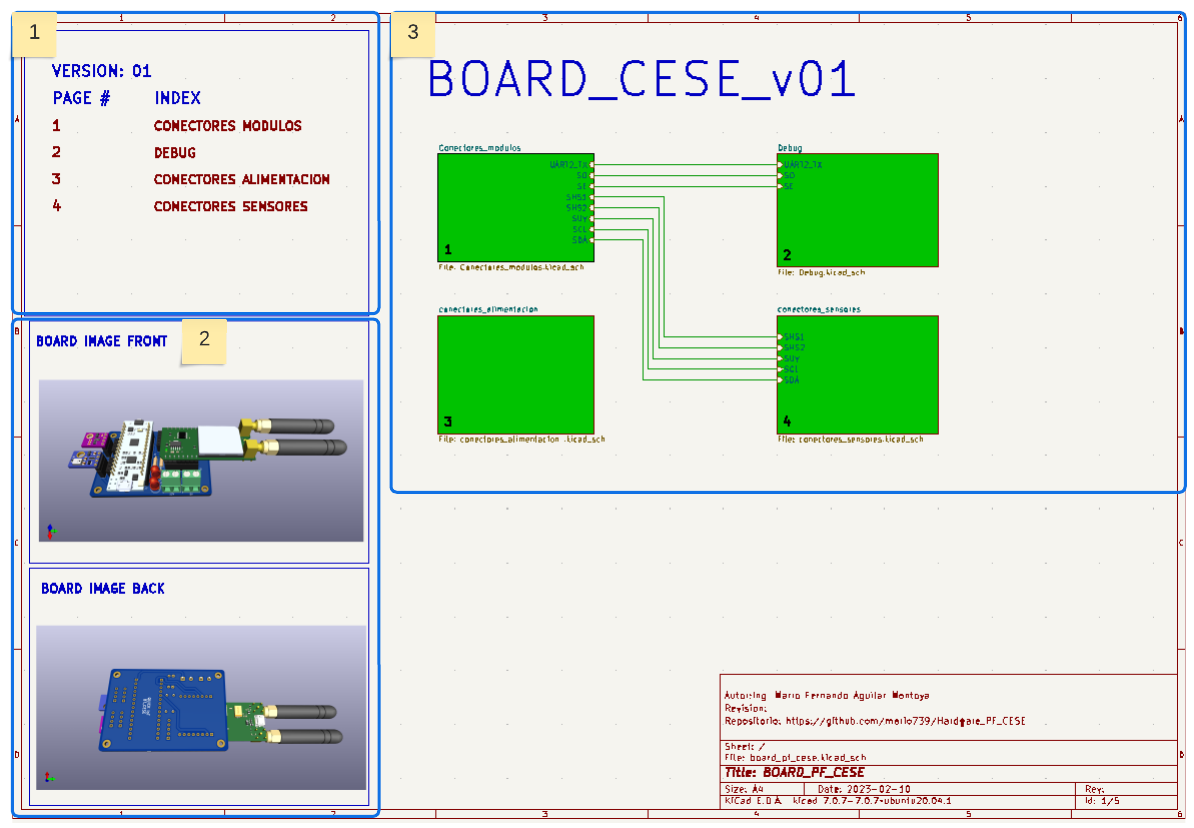
\includegraphics[width=\textwidth, height=8.5cm]{./Figures/esquematico_raiz.png}
	\caption{Esquemático página raíz.}
	\label{fig:esquematico root}
\end{figure}

En figura \ref{fig:esquematico modulos} se muestran los conectores de los módulos más importantes: el módulo de comunicación BG96, módulo NUCLEO-L432KC y la conexión entre ellos.

\begin{figure}[h]
  \centering
	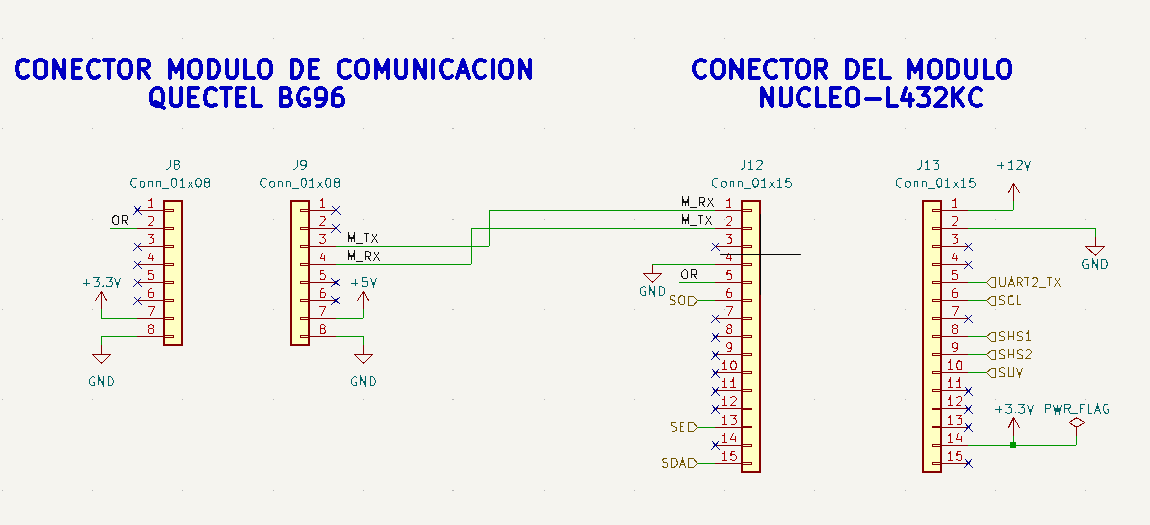
\includegraphics[width=10cm, height=3.5cm]{./Figures/esquematico_modulos.png}
	\caption{Conector módulo BG96 y NUCLEO-L432KC.}
	\label{fig:esquematico modulos}
\end{figure}

Se colocaron dos leds para debug, uno para señalizar si se logró conectar al servidor MQTT y el otro led para señalizar si el sistema entra en un estado de error. Se colocó un conector para una puerto serial por donde el módulo manda la secuencias de comandos que manda y recibe del módulo de comunicación. En la figura \ref{fig:esquematico conectores de debug} se puede ver el circuito.
\begin{figure}[h!]
  \centering
	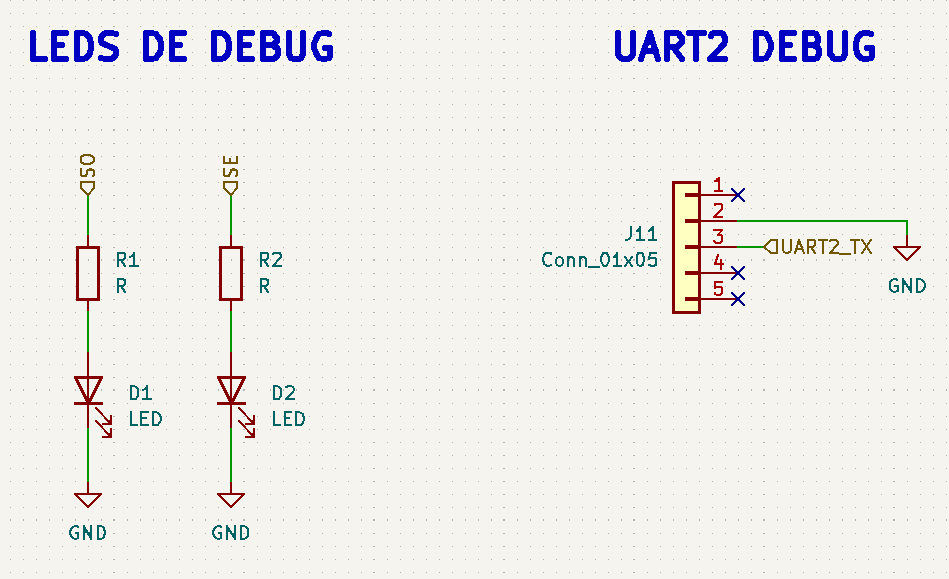
\includegraphics[width=10cm, height=4cm]{./Figures/esquematico_debug.png}
	\caption{Esquemático interfaz de debug.}
	\label{fig:esquematico conectores de debug}
\end{figure}

En la figura \ref{fig:esquematico conectores sensores} se pueden ver los conectores que se colocaron a la placa para conectar los sensores del nodo: sensor de humedad 1, sensor de humedad 2, sensor de luz UV y el sensor de humedad y temperatura ambiente AHT-10.
\begin{figure}[h]
  \centering
	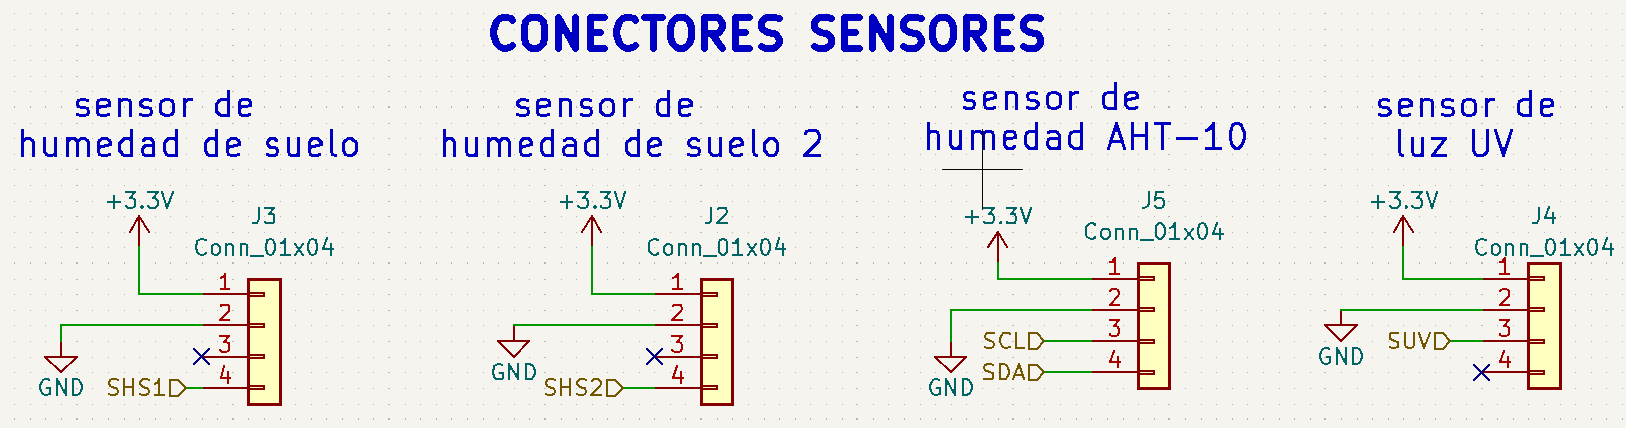
\includegraphics[width=10cm, height=4.5cm]{./Figures/conectores_sensores.png}
	\caption{Esquemático conectores sensores.}
	\label{fig:esquematico conectores sensores}
\end{figure}

Se colocaron dos colectores de alimentación como se muestra en la figura \ref{fig:esquematico conectores alimentacion}, el conector de 12V para alimentar al módulo del microcontrolador y el otro conector para alimentar al módulo de comunicación.
\begin{figure}[h]
  \centering
	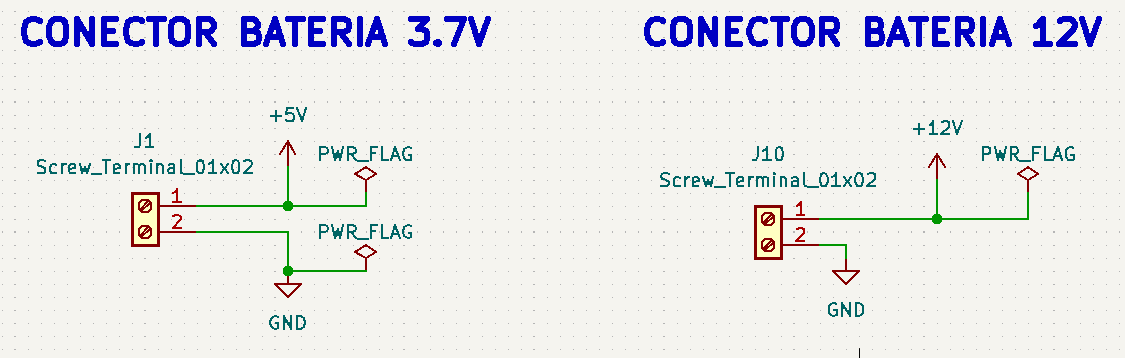
\includegraphics[width=10cm, height=4.5cm]{./Figures/esquematico_alimentacion.png}
	\caption{Esquemático conectores alimentación.}
	\label{fig:esquematico conectores alimentacion}
\end{figure}

\subsection{PCB del hardware} 
La figura \ref{fig:PCB del proyecto} muestra el circuito impreso diseñado para el proyecto.

\begin{figure}[h!]
  \centering
  \begin{subfigure}[b]{0.28\linewidth}
  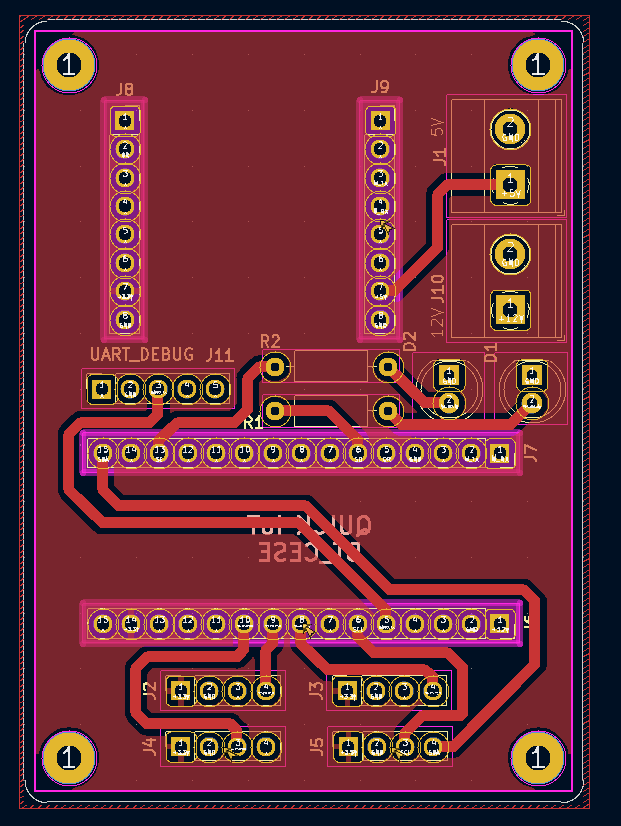
\includegraphics[width=\linewidth]{./Figures/pcb_top.png}
  \caption{Capa top PCB}
  \label{fig:Capa top PCB}
  \end{subfigure}
  \begin{subfigure}[b]{0.27\linewidth}
  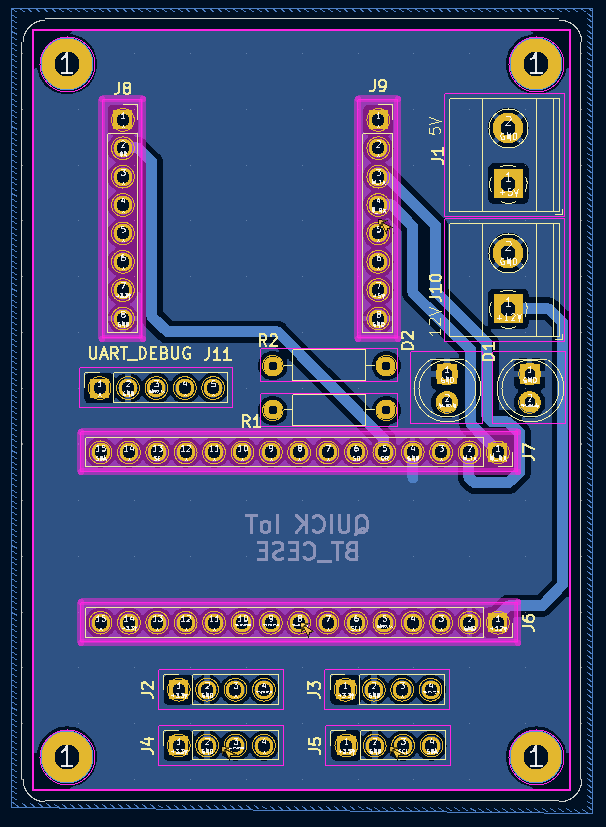
\includegraphics[width=\linewidth]{./Figures/pcb_bot.png}
  \caption{Capa bot PCB}
  \label{fig:Capa bot PCB}
  \end{subfigure}
  \caption{PCB del proyecto.}
  \label{fig:PCB del proyecto}
\end{figure}

En la figura \ref{fig:3D del modulo} se muestra el diseño de la tarjeta del circuito impreso en 3D.
\begin{figure}[h!]
  \centering
	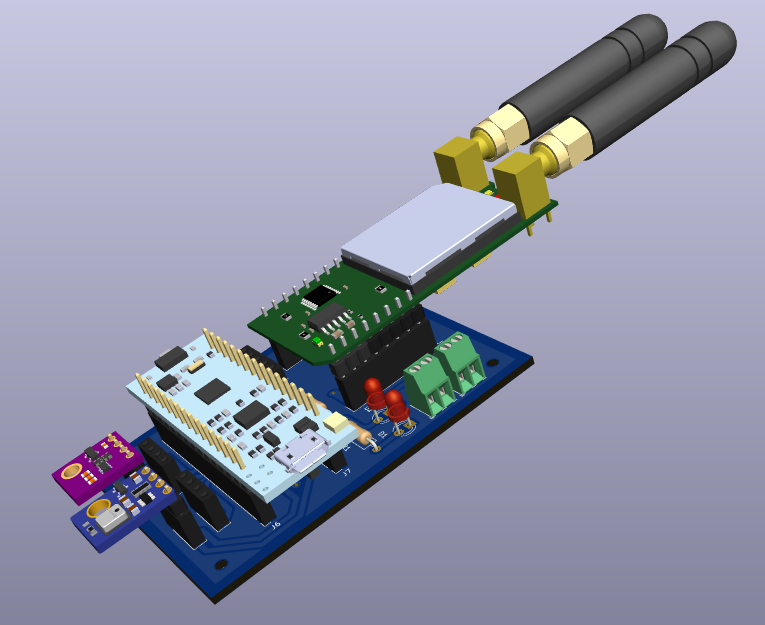
\includegraphics[width=8cm, height=4.5cm]{./Figures/tarjeta3d.png}
  \caption{Modelo 3D de la tarjeta.}
	\label{fig:3D del modulo}
\end{figure}
\subsection{Fabricación circuito impreso} 
Una vez completado y validado el diseño, se generaron los archivos de fabricación y se mandaron a la empresa JLCPCB parar su producción. La figura \ref{fig:PCB ensamblado} muestra la tarjeta ya ensamblada con los módulos. 
\begin{figure}[h!]
  \centering
	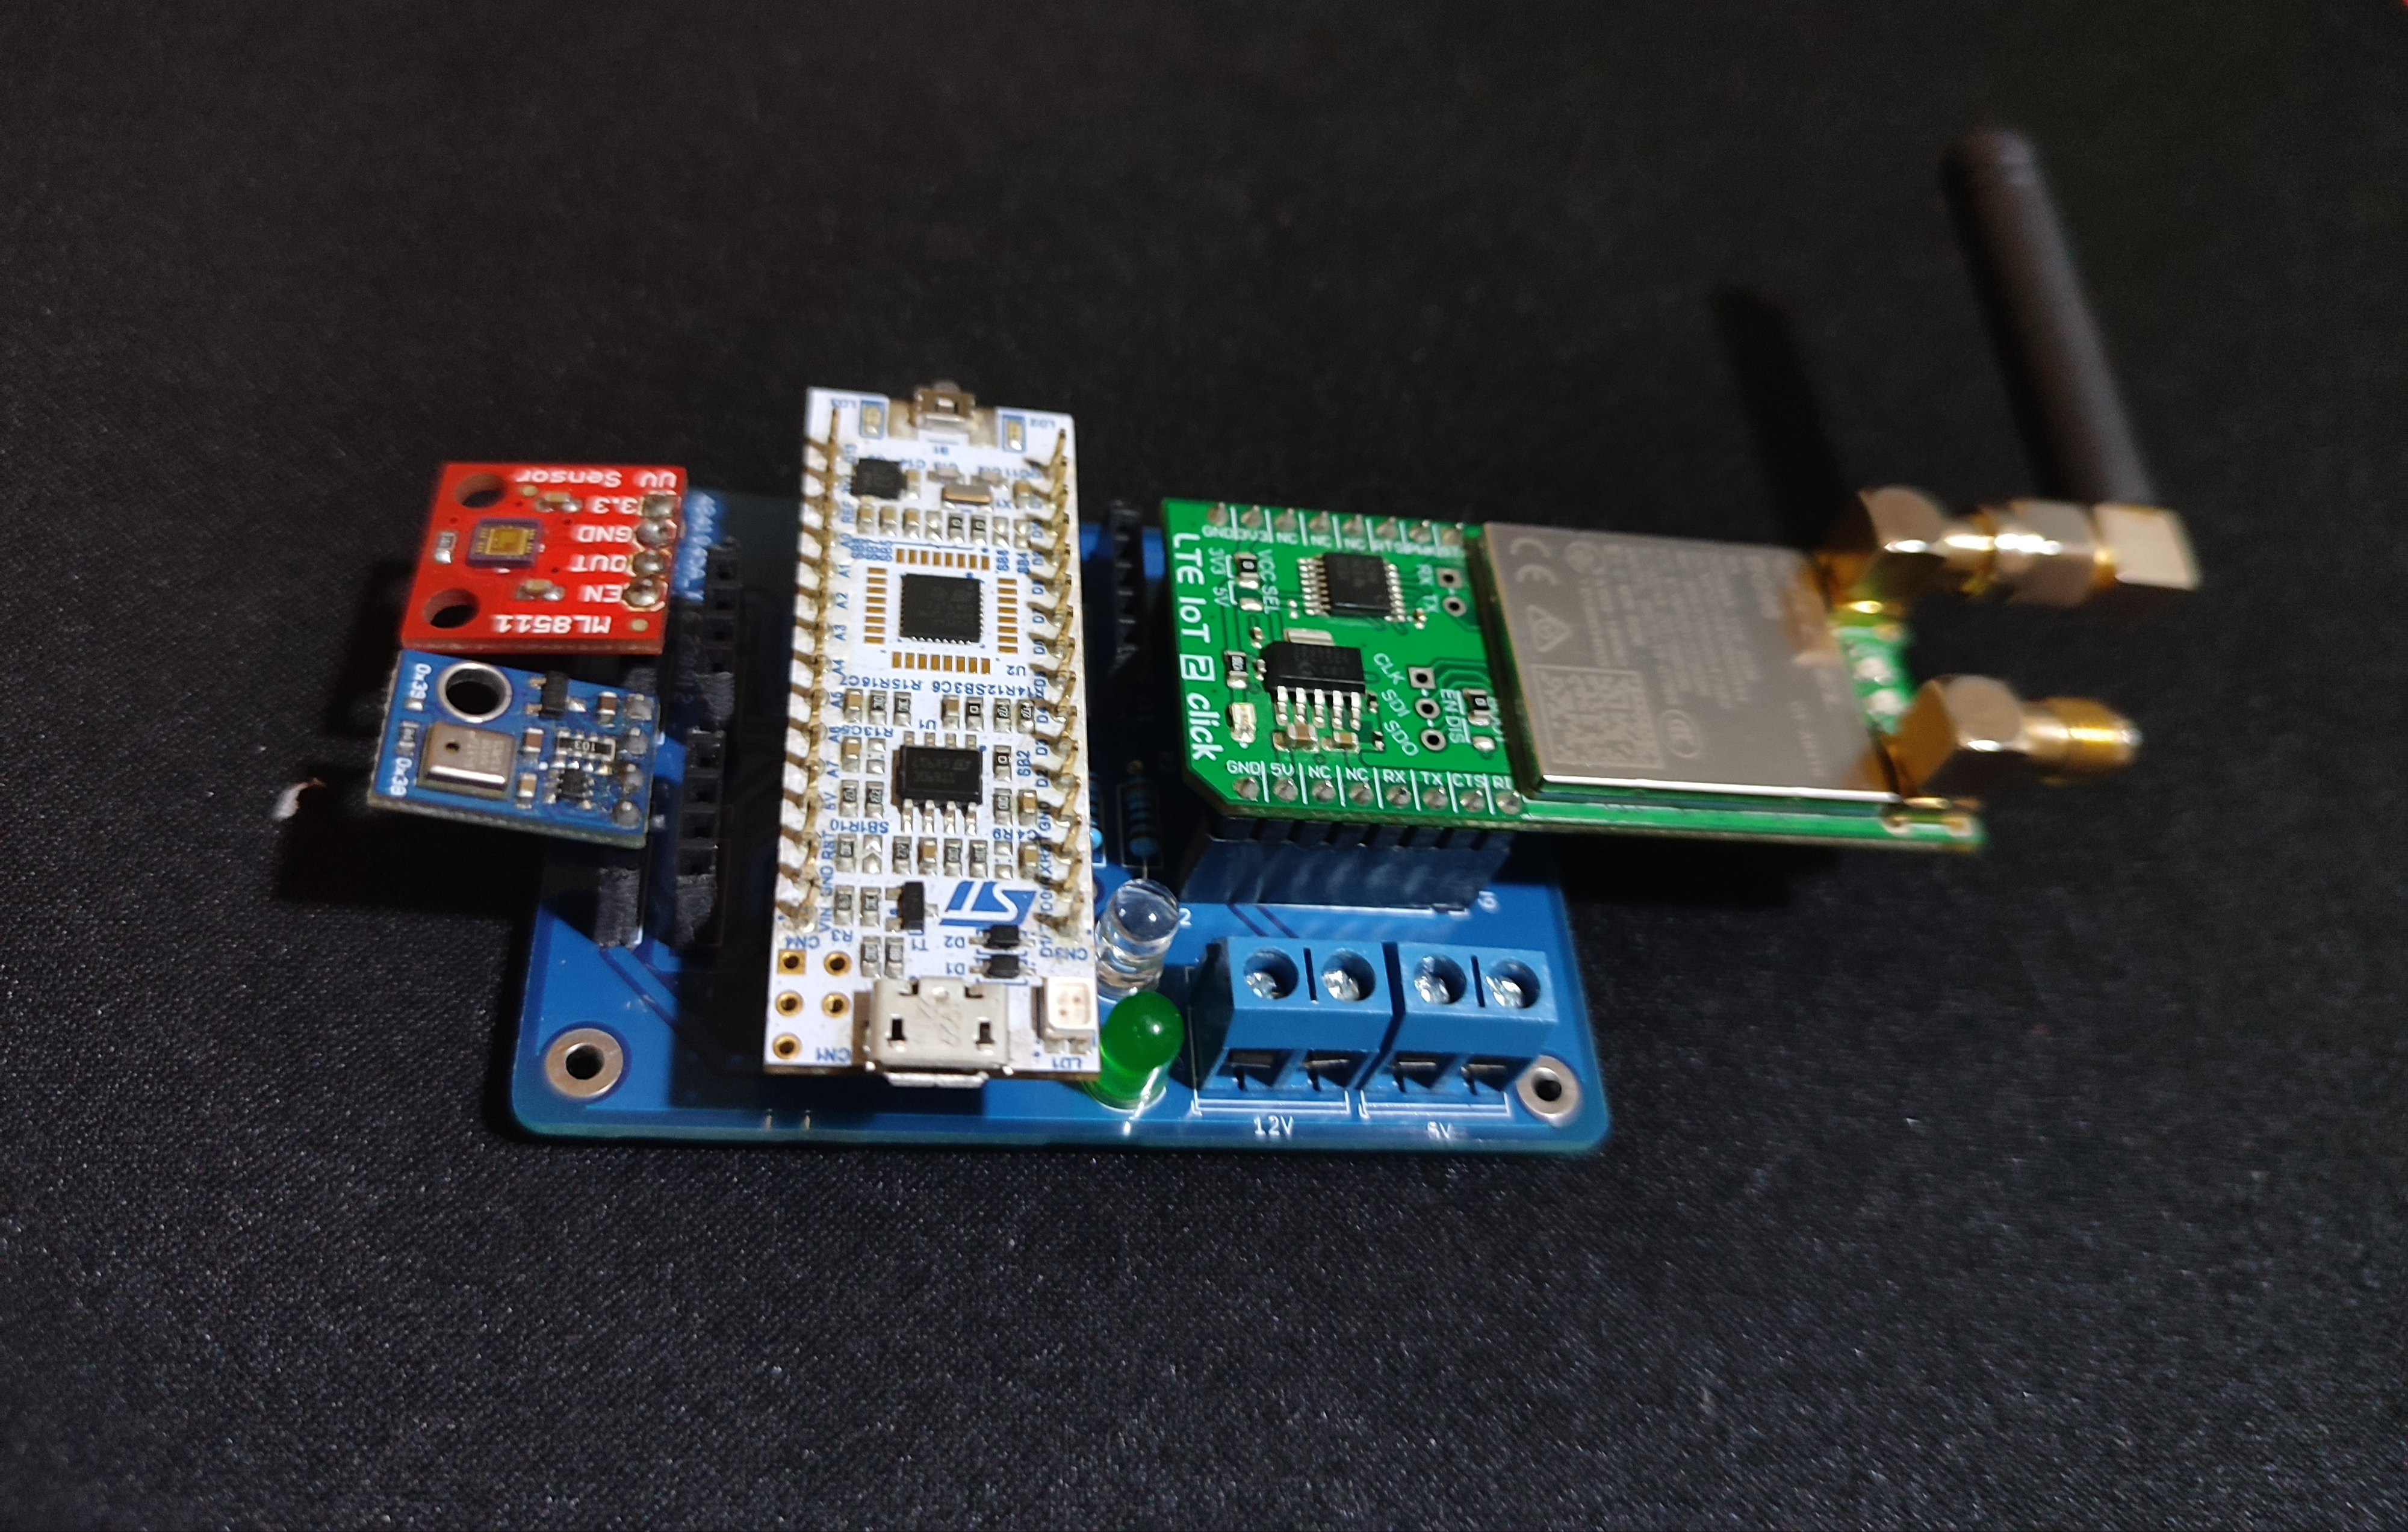
\includegraphics[width=8cm, height=5cm]{./Figures/hardware_vistalateral.jpg}
  \caption{PCB ensamblado.}
	\label{fig:PCB ensamblado}
\end{figure}

\clearpage
\section{Paneles de visualización}
La herramienta de visualización de ThingsBoard es muy versátil para el armado de paneles de visualización escalables y altamente configurables.

Se armó un panel de visualización principal que muestra los nodos sensores monitoreados por el sistema y un panel secundario que muestra las variables monitoreadas por cada nodo sensor a través gráficas, tablas, etc.

\subsection{Panel principal} 

En la figura \ref{fig:Panel principal} se aprecia el panel principal de la interfaz gráfica. A continuación se describirán cada zona del panel principal.
El panel está dividido en las siguientes zonas:
\begin{itemize}
  \item Zona 1: listado de todos los nodos sensores implementados y activos, haciendo click en el sensor se navega al panel de visualización secundario.
  \item Zona 2: gráficas que muestra los cambios que van teniendo los valores de las variables medidas por los sensores con respecto al tiempo.
  \item Zona 3: mapa con la ubicación de los nodos sensores implementados.
\end{itemize}

\begin{figure}[h]
  \centering
	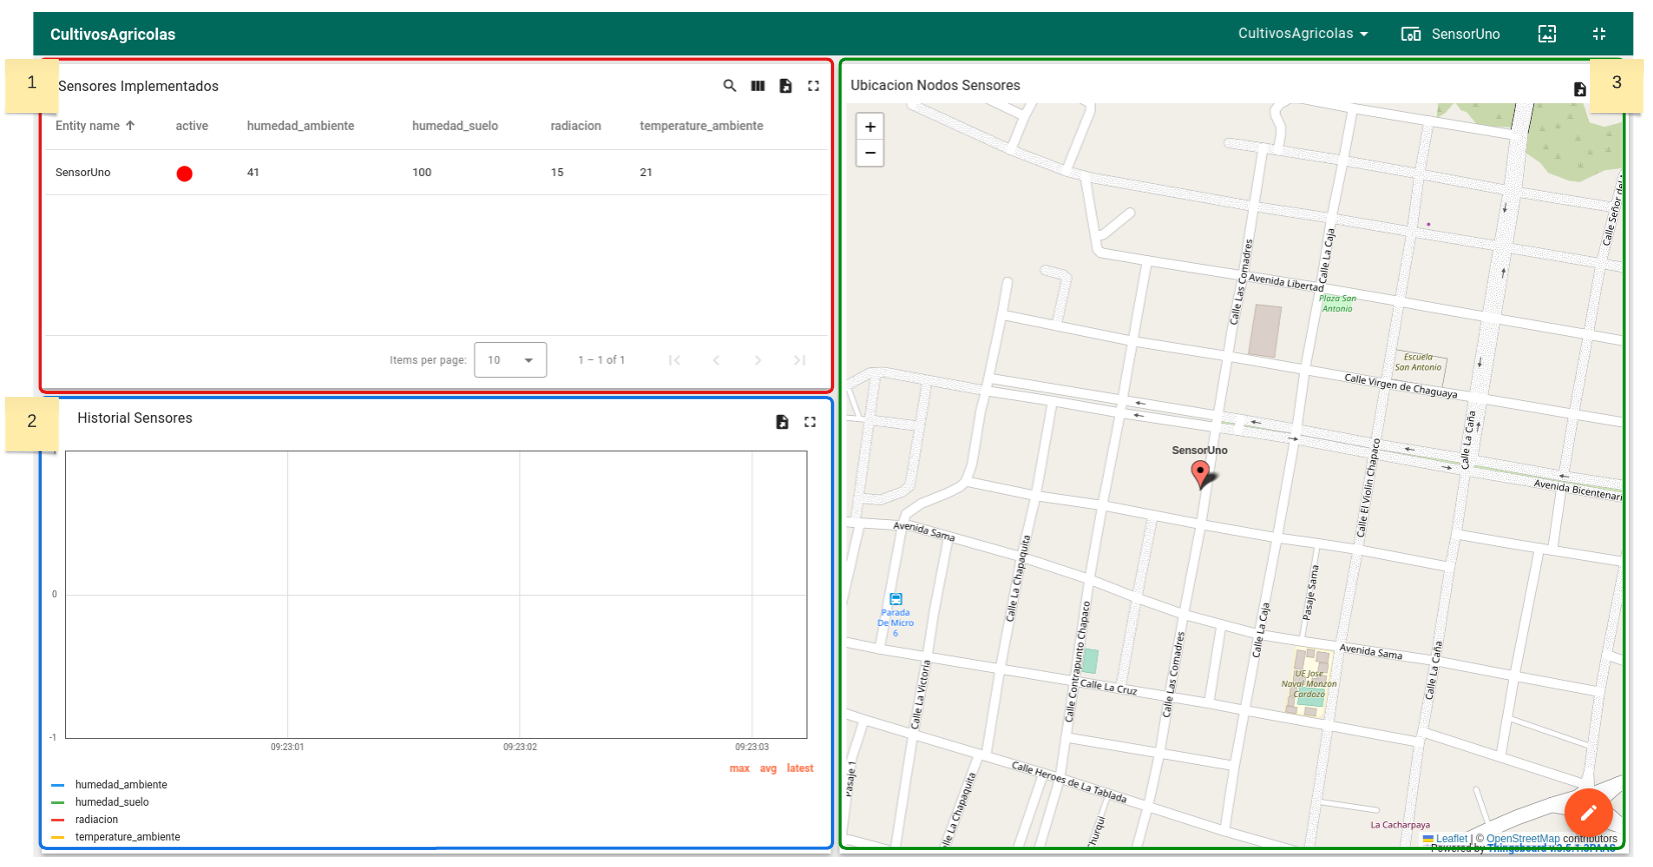
\includegraphics[width=\textwidth, height=10cm]{./Figures/panel_principal_editado.png}
  \caption{Panel principal de la interfaz gráfica.}
	\label{fig:Panel principal}
\end{figure}

\clearpage
\subsection{Panel nodo sensor} 

Para tener un mayor detalle de todos los parámetros de monitoreo de cada nodo sensor se creó un panel secundario que se muestra en la figura \ref{fig:Panel nodo sensor}.

El panel está dividido en las siguientes zonas:
\begin{itemize}
  \item Zona 1: gráficas que muestran los cambios que van teniendo los valores de las variables medidas por los sensores con respecto al tiempo.
  \item Zona 2: widgets que muestran el último valor obtenido por el nodo sensor de cada variable monitoreada.
  \item Zona 3: tabla que muestra las alarmas que se activaron. 
  \item Zona 4: se tiene un mapa que muestra la ubicación del nodo sensor implementado.
\end{itemize}

\begin{figure}[h!]
  \centering
	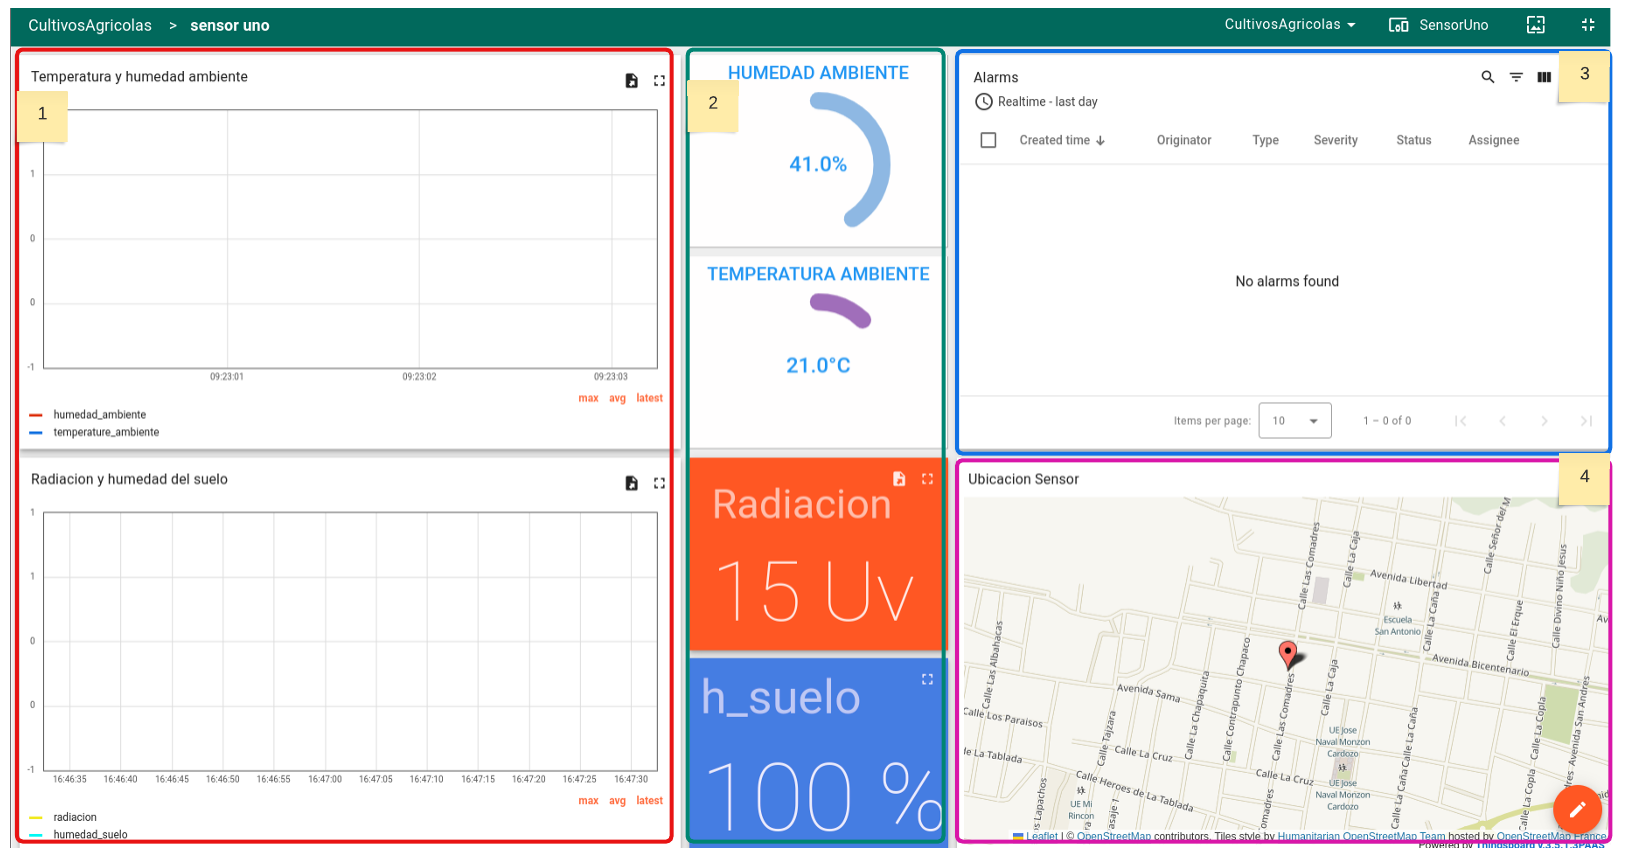
\includegraphics[width=\textwidth, height=10cm]{./Figures/panel_nodosensor_editado.png}
  \caption{Panel nodo sensor.}
	\label{fig:Panel nodo sensor}
\end{figure}